\chapter{Algorithmes issus de la programmation par contraintes pour le
\CECSP}
\label{sec:PPC_CECSP}
Dans ce chapitre, nous décrivons des algorithmes et modèles issus de
la programmtion par contrainte. Les deux premières sections sont
dédiées à la présentation d'algorithmes de filtrage pour le problème
de décision du \CECSP. En effet, comme dans le cas du \CUSP, la
NP-complétude de ce problème implique qu'un algorithme assurant la
cohérence des bornes de chaque variable - assurant l'existance d'une
solution où les valeurs de chaque variables sont comprises dans ces
bornes - ne peut s'exécuter en temps polynomial. Par conséquent,
plusieurs relaxations sont proposées afin de supprimer les valeurs
possibles de début et fin de tâches
incohérentes en temps polynomial. 

Les premières relaxations présentées sont basées sur le raisonnement
Time-table pour le \CUSP, décrit dans le
paragraphe~\ref{sec:cumu_propag}, tandis que la dernière se base sur
le raisonnement énergétique défini pour ce même problème.

Dans un second temps, nous présentons un modèle de programmation par
contraintes permettant de résoudre le \CECSP~ discret, i.e. où les
variables ne peuvent prendre que des valeurs discrètes. 

%%% Local Variables:
%%% mode: latex
%%% TeX-master: "../main_file"
%%% End:

\section{Algorithmes de filtrage basés sur le Time-Table}

La section suivante présente plusieurs algorithmes de filtrage pour le
\CECSP. Tous ces algorithmes utilisant une adaptation du Time-Table
pour le \CUSP, nous commençons donc par présenter brièvement comment
ce raisonnement est modifié pour être adapté dans le cadre du \CECSP.
Puis, nous présentons deux autres algorithmes permettant
de réduire l'ensemble des valeurs possibles pouvant être prises par
chaque variable. Le premier est adapté du Time-Table disjonctif pour
le \CUSP~\cite{Gay2015} et le dernier utilise une combinaison entre
problème de flots et profil obligatoire.

\subsection{Le Time-Table}
\index{Time-Table!CECSP}
Comme pour le \CUSP, le Time-Table pour le \CECSP~se base sur la
notion de partie obligatoire des activités, i.e. l'intervalle pendant
lequel une activité est en cours d'exécution dans tous les
ordonnancements réalisables. Cependant, comme dans le cas du \CECSP,
nous ne connaissons pas la durée exacte d'une activité, nous utilisons
une borne inférieure sur sa durée pour calculer la date de début au
plus tard, $\LS$, et la date de fin au plus tôt, $\EE$. Pour calculer
cette borne, remarquons que la configuration permettant de finir une
activité le plus rapidement possible, est celle où l'activité est
exécutée à son rendement maximal $\bmax$. De ce fait, une borne
inférieure sur la durée de l'activité vaut $W_i/f_i(\bmax)$. Nous
pouvons donc calculer la date de début au plus tard de l'activité,
$\LS=d_i-W_i/f_i(\bmax)$, et sa date de fin au plus tôt,
$\EE=r_i+W_i/f_i(\bmax)$. La partie obligatoire d'une activité $i$ est
alors définie de a même manière que pour le \CUSP, i.e la partie
obligatoire de $i$ est l'intervalle $[\LS,\EE]$
(cf. figure~\ref{fig_mand_CECSP}).

Cependant, dans le cas où $\LS \le \EE$, i.e. où l'activité possède
une partie obligatoire, nous pouvons seulement déduire que l'activité
$i$ va consommer au moins une quantité $\bmin$ de la ressource durant
toute sa partie obligatoire, et ce, quelque soit le moment où
l'activité est ordonnancée. La notion de profil obligatoire de la
ressource est donc légèrement différente de celle définie pour le
\CUSP~(cf. définition~\ref{def:profil_oblig},
page~\pageref{def:profil_oblig}).

\begin{defi}
Le profil obligatoire d'une ressource $TT_{\A}$ dans le cas du
\CECSP~est définie de la façon suivante: 
\[TT_{\A}(t)=\sum_{\substack{i \in \A\\\LS \le t \le \EE}} \bmin\quad
  \forall t \in \H\]
Le problème est donc insatisfiable dans le cas où $\exists t \in \H\
:\ TT_{\A}(t) > R$
\end{defi}

\begin{ex}
Considérons l'activité suivante: 

\vspace{-0.5cm}
\begin{center}
  \begin{tabular}{|P{1cm}P{1cm}P{1cm}P{1cm}P{1cm}P{1cm}|}
    \hline
    \ES & \LE & W_i & \bmin & \bmax & f_i(b)\\
    \hline
    1 & 14 & 72 & 2 & 5 & b+3\\
    \hline
  \end{tabular}
\end{center}

Nous pouvons calculer sa date de début au plus tard,
$\LS=d_i-W_i/f_i(\bmax)=14 - 72/8 =5$, ainsi que sa date de fin au
plus tôt, $\EE=r_i+ W_i/f_i(\bmax)=1 + 72/8 =10$. Comme $\EE > \LS$,
l'activité possède une partie obligatoire qui est l'intervalle
$[5,10]$ (voir
figure~\ref{fig_mand_CECSP_a},~\ref{fig_mand_CECSP_b}). Cependant,
nous pouvons seulement en déduire que l'activité sera en cours dans
cet intervalle et ,grâce à la borne inférieure sur la quantité de
ressource que peut consommer l'activité durant son exécution, nous
pouvons déduire que, sur l'intervalle $[\LS,\EE]$, l'activité est au
moins exécutée à $\bmin$ (voir figure~\ref{fig_mand_CECSP_c}).
  
\begin{figure}[htb!]
\vspace{-0.8cm}
\subcaptionbox{Ordonnancement au plus tôt\label{fig_mand_CECSP_a}}[0.3\linewidth]{
    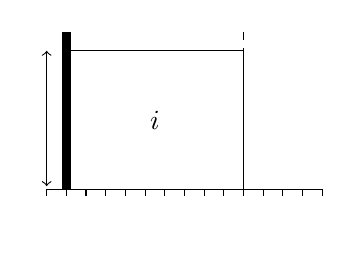
\begin{tikzpicture}
      [xscale=0.25, yscale= 0.4,node distance=0.5cm]
      \node (sil) at (1,0) {} ;
      \node (eil) at (10,0) {} ;
      \node [below of=eil,node distance=0.63cm]  {$\EE$};
      \draw (sil.center) node[below=0.2cm] {$\ES$};
      
      \draw (0,0) -- (14,0);
      \draw[line width=3pt] (1,0) -- (1,5);
      
      \draw[<->] (0,0.1) -- (0,4.4) node[midway,left] {$\bmax$};
      \draw (1,0) rectangle (10,4.4) node[midway] {$i$};

      \draw[dashed] (10,0) -- (10,5);

      \foreach \i in {0,...,14} {
        \draw (\i,0)  -- (\i,-0.2);
      }
    \end{tikzpicture}
}
\hfill
\subcaptionbox{Ordonnancement au plus tard\label{fig_mand_CECSP_b}}[0.3\linewidth]{
    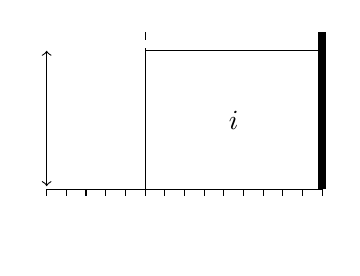
\begin{tikzpicture}
      [xscale=0.25, yscale= 0.4,node distance=0.5cm]
      \node (sir) at (5,0) {} ;
      \node (eir) at (14,0) {} ;
      \node[below of= sir,node distance=0.63cm] {$\LS$};
      \draw (eir.center) node[below=0.2cm] {$\LE$};
      
      \draw (0,0) -- (14,0);
      \draw[line width=3pt] (14,0) -- (14,5);
      
      \draw[<->] (0,0.1) -- (0,4.4) node[midway,left] {$\bmax$};
      \draw (5,0) rectangle (14,4.4) node[midway] {$i$};

      \draw[dashed] (5,0) -- (5,5);

      \foreach \i in {0,...,14} {
        \draw (\i,0)  -- (\i,-0.2);
      }
    \end{tikzpicture}
}
\hfill
\subcaptionbox{Ordonnancement réalisable à $\bmin$ dans
  $[\LS,\EE]$ \label{fig_mand_CECSP_c}}[0.3\linewidth]{ 
    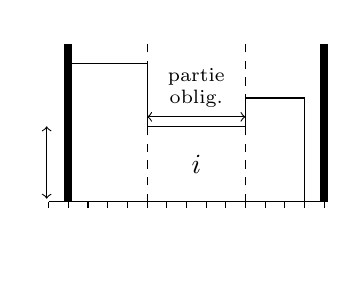
\begin{tikzpicture}
      [xscale=0.25, yscale= 0.4,node distance=0.5cm]
      \node (sir) at (5,0) {} ;
      \node (eil) at (10,0) {} ;
      \node [below of=eil,node distance=0.63cm]  {$\EE$};
      \node[below of= sir,node distance=0.63cm] {$\LS$};
      \draw[<->] (5,2.7) -- (10,2.7) node[midway,above,text width=1.4cm]
      {\begin{center} \scriptsize partie oblig. \end{center}};
      
      \draw[white] (5,0) rectangle (10,2.4) node[midway,color=black] {$i$};
           
      \draw (1,4.4) -- (5,4.4) -- (5,2.4) -- (10,2.4) -- (10,3.3) --
      (13,3.3) -- (13,0);
      
      \draw (0,0) -- (14,0);
      \draw[line width=3pt] (1,0) -- (1,5);
      \draw[line width=3pt] (14,0) -- (14,5);
      
      \draw[<->] (-0.1,0.1) -- (-0.1,2.4) node[midway,left] {$\bmin$};
    


      \draw[dashed] (5,0) -- (5,5);
      \draw[dashed] (10,0) -- (10,5);

      \foreach \i in {0,...,14} {
        \draw (\i,0)  -- (\i,-0.2);
      }
    \end{tikzpicture}
}
\caption{Partie obligatoire d'une activité $i$}
\label{fig_mand_CECSP}
\end{figure}
\end{ex}

Le profil obligatoire peut aussi être calculé en $O(n)$ à l'aide d'un
algorithme de balayage en triant au préalable les activités par date
de début au plus tard et date de fin au plus tôt.

Nous détaillons maintenant l'adaptation du Time-Table disjonctif au
\CECSP. 

\subsection{Le Time-Table disjonctif}

Le second algorithme de filtrage proposé repose sur un raisonnement
appelé Time-Table disjonctif et utilisé, en premier lieu, pour le
\CUSP (cf. paragraphe~\ref{sec:mix_CUSP}). Ce dernier repose sur le
raisonnement Time-Table décrit précédemment et sur le raisonnement
disjonctif.

Le raisonnement disjonctif dans le cadre du \CECSP, est très similaire
à celui défini pour le \CUSP. La différence repose sur la construction
des ensembles disjonctifs. Dans le cas du \CECSP, un couple
d'activités ($i,j)$ sera dit disjonctif si $\bmin+\bmin[j] >R$. Dans
ce cas, nous savons que:
\begin{itemize}
\item l'activité $i$ doit commencer après l'activité $j$, ou, 
\item l'activité $i$ doit finir avant l'activité $j$.  
\end{itemize}

Cette propriété permet, entre autre, d'ajuster la date de début au
plus tôt de $j$. En effet, $\ES[j] \le \EE$ et $\LS \le \EE[j]$
implique que $j$ doit commencer après la fin de l'activité $i$ (voir
figure~\ref{fig:disj_CECSP}). De ce fait, la début de $j$ ne peut arriver
avant la date de fin au plus tôt de $i$, et donc: $\ES[j] \ge \EE$. La
règle de filtrage est ensuite similaire à celle mise en place pour le
\CUSP. 

\begin{reg}
Soient $i, j \in \A, i \neq j$ telles que $\bmin+\bmin[j] < R$ et $\LS
< \EE[j]$. Alors la date de début au plus tôt de l’activité peut être
ajustée et on a : $\ES[j] \ge \EE$.
\end{reg}

\begin{ex}
Considérons les deux activités suivantes: 
\begin{center}
\begin{tabular}{|P{1cm}|P{1cm}P{1cm}P{1cm}P{1cm}P{1cm}P{2cm}|}
    \hline
    act & \ES & \LE & W_i & \bmin & \bmax & f_i(b_i(t))  \\
    \hline
   i & 2 & 11 & 28 & 2 & 3 & 2*b_i(t) +1\\
   j & 1 & 20 & 49 & 2 & 4 & voir fig~\ref{fig:fonct_CECSP}\\
    \hline
  \end{tabular}
\end{center}

La fonction $f_j(b)$ est définie par l'expression suivante: 
\[f_j(b)=\left\{
\begin{array}{lll}
2b & & b \in [2,3]\\
b+3 & & b \in [3,4]
\end{array}
\right.\] 
et décrite dans la figure~\ref{fig:fonct_CECSP}
\begin{figure}[!htb]
\centering
\begin{tikzpicture}
[xscale=0.8,yscale=0.56]
\node (O) at (1,2) {};
\draw[->] (1,2) -- (5.5,2);
\draw[->] (1,2) -- (1,8);

\path[draw] (2,4) -- (3,6) -- (4,7) ;

\draw[dotted] (2,2) node[below] {\footnotesize $2$} -- (2,8);
\draw[dotted,color=gray!70] (4,2) node[below,color=black] {\footnotesize $4$}
-- (4,8);
\draw[dotted] (3,2) node[below] {\footnotesize $3$} -- (3,8);

\draw (1,4) node[left] {\footnotesize $4$};
\draw (1,6) node[left] {\footnotesize $6$};
\draw (1,7) node[left] {\footnotesize $7$};
\end{tikzpicture}
\caption{Fonction $f_j(b_j(t))$}
\label{fig:fonct_CECSP}
\end{figure}

Dans cet exemple, comme $\bmin +\bmin[j] =4 > 3$, $i$ et $j$ ne
peuvent s'exécuter en parallèle. Si l'activité $i$ finit au temps
$\LE= 11$ alors, elle chevauche forcément l'activité $j $ (voir
figure~\ref{fig:disj_CECSPa} et~\ref{fig:disj_CECSPb}). Dans tous
ordonnancement réalisable, $i$ est donc exécuté avant $j$ et la date de
début au plus tôt de $j$ peut donc être ajustée, i.e. $j$ ne peut
commencer avant $\EE=6$ (voir
figure~\ref{fig:disj_CECSPc}).
  \begin{figure}[htb!] 
    \subcaptionbox{Si $i$ finit au temps $11$...\label{fig:disj_CECSPa}}[0.45\linewidth]{
    \centering
    \begin{tikzpicture} [yscale=0.4,xscale=0.4]   
        \node (O) at (0,0) {};
      \foreach \i in {0,5,...,10} {
        \draw (\i,0) -- (\i,-0.1) node[below] {\small $\i$};
      }
      \fill[gray!50] (2,0) rectangle (11,3.4);
      \fill[gray!50] (1,3.6) rectangle (14,8);
      
      \draw[fill=white] (6.4,0.2) -- (6.4,3.2)   -- (8.4,3.2) -- (8.4,2) --node[midway,below=0.2cm] {$i$}
      (11,2) -- (11,0.2) -- cycle;
      
      \draw[fill=white] (1,3.8) -- (1,7.8)  node[midway,right=0.6cm] {$j$} -- (6,7.8) -- (6,5.8) --
      (9.5,5.8) -- (9.5,3.8) -- cycle;
      \draw[white, pattern=north west lines] (6.4,0) rectangle (9.5,8);

      \draw[->] (0,0) -- (14,0);
      \draw[->] (0,0) -- (0,8) ;
      \draw (0,3) node[left] {$R=3$};
      \draw[densely dotted] (1,-0.1) -- (1,8) node[above] {$\ES[j]$};
      \draw[densely dotted] (8,-0.1) -- (8,8) node[above] {$\EE[j]$};
      \draw[densely dotted] (2,-0.1)  node[below] {$\ES$}-- (2,8);
      \draw[densely dotted] (6,-0.1 ) node[below=0.4cm] {$\EE$}-- (6,8) ;
      \draw[densely dotted] (7,-0.1) node[below] {$\LS$} -- (7,8) ;
      \draw[densely dotted] (11,-0.1) node[below right] {$\LE$} -- (11,8) ;
      \draw[<->] (14.5,0.2) -- (14.5,3.2) node[midway,right] {$\bmax$} ;
      \draw[<->] (14.5,3.8) -- (14.5,7.8) node[midway,right] {$\bmax[j]$} ;   
    \end{tikzpicture}
  }
    \subcaptionbox{...alors $i$ chevauche forcément l'activité $j$\label{fig:disj_CECSPb}}[0.45\linewidth]{
        \centering
        \begin{tikzpicture}[yscale=0.4,xscale=0.4]
      \node (O) at (0,0) {};
      \foreach \i in {0,5,...,10} {
        \draw (\i,0) -- (\i,-0.1) node[below] {\small $\i$};
      }
      \fill[gray!50] (2,0) rectangle (11,3.4);
      \fill[gray!50] (1,3.6) rectangle (14,8);
      
      \draw[fill=white] (7,0.2) rectangle (11,3.2) node[midway]
      {$i$};
      \draw[fill=white] (1,3.8) rectangle (8,7.8) node[midway]
      {$j$};
      \draw[white, pattern=north west lines] (7,0) rectangle (8,8);

      \draw[->] (0,0) -- (14,0);
      \draw[->] (0,0) -- (0,8) ;
      \draw (0,3) node[left] {$R=3$};
      \draw[densely dotted] (1,-0.1) -- (1,8) node[above] {$\ES[j]$};
      \draw[densely dotted] (8,-0.1) -- (8,8) node[above] {$\EE[j]$};
      \draw[densely dotted] (2,-0.1)  node[below] {$\ES$}-- (2,8);
      \draw[densely dotted] (6,-0.1 ) node[below=0.4cm] {$\EE$}-- (6,8) ;
      \draw[densely dotted] (7,-0.1) node[below] {$\LS$} -- (7,8) ;
      \draw[densely dotted] (11,-0.1) node[below right] {$\LE$} -- (11,8) ;
      % \draw[densely dotted] (6,-0.1) -- (6,8) node[above] {$\ES[j]^{'}$};
      % \draw[->] (1.8,5.8) -- (5.2,5.8);
      \draw[<->] (14.5,0.2) -- (14.5,3.2) node[midway,right] {$\bmax$} ;
      \draw[<->] (14.5,3.8) -- (14.5,7.8) node[midway,right]
      {$\bmax[j]$} ;
    \end{tikzpicture}
   }
    \subcaptionbox{$\ES[j]$ peut être ajusté\label{fig:disj_CECSPc}}[\linewidth]{    \centering
      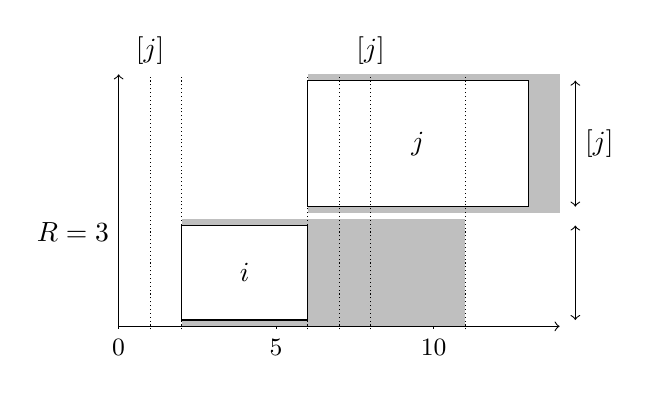
\begin{tikzpicture} [yscale=0.4,xscale=0.4]
      \node (O) at (0,0) {};
      \foreach \i in {0,5,...,10} {
        \draw (\i,0) -- (\i,-0.1) node[below] {\small $\i$};
      }
      \fill[gray!50] (2,0) rectangle (11,3.4);
      \fill[gray!50] (6,3.6) rectangle (14,8);
      
      \draw[fill=white] (2,0.2) rectangle (6,3.2) node[midway]
      {$i$};
      \draw[fill=white] (6,3.8) rectangle (13,7.8) node[midway]
      {$j$};

      \draw[->] (0,0) -- (14,0);
      \draw[->] (0,0) -- (0,8) ;
      \draw (0,3) node[left] {$R=3$};
      \draw[densely dotted] (1,-0.1) -- (1,8) node[above] {$\ES[j]$};
      \draw[densely dotted] (8,-0.1) -- (8,8) node[above] {$\EE[j]$};
      \draw[densely dotted] (2,-0.1)  node[below] {$\ES$}-- (2,8);
      \draw[densely dotted] (6,-0.1 ) node[below=0.4cm] {$\EE$}-- (6,8) ;
      \draw[densely dotted] (7,-0.1) node[below] {$\LS$} -- (7,8) ;
      \draw[densely dotted] (11,-0.1) node[below right] {$\LE$} -- (11,8) ;
      \draw[<->] (14.5,0.2) -- (14.5,3.2) node[midway,right] {$\bmax$} ;
      \draw[<->] (14.5,3.8) -- (14.5,7.8) node[midway,right] {$\bmax[j]$} ;

  \end{tikzpicture}
}
  \caption{Raisonnement disjonctif}
  \label{fig:disj_CECSP}
\end{figure}
\end{ex}

Nous pouvons maintenant présenter l'adaptation du Time-Table
disjonctif au cas du \CECSP. Pour ce faire, nous commençons par
adapter la définition d'intervalle minimum de superposition, puis nous
présenterons les modifications apportées aux règles d'ajustement du
\CUSP~afin que ces dernières soient applicables dans le cas du
\CECSP. Enfin, l'extension de ces règles dans le cas où les activités
ne possèdent pas de partie obligatoire sera décrit. Cette extension
n'avait pas été présentée dans le chapitre sur le \CUSP~mais est
décrite dans l'article~\cite{Gay2015}. 

La notion d'intervalle minimum de superposition s'adapte naturellement
au cas du \CECSP. En effet, cette intervalle représente l'ensemble
minimal de points de temps tel que une activité $i$ est forcément en
cours durant un de ces points. 

\begin{defi}
\label{des:moi_CUSP} 
Soit $\EE^{-}$ le point le plus proche de $\EE$, i.e. $\forall \delta
>0 , |\EE^{-} -\EE| \le \delta$. L'intervalle minimum de
superposition d'une activité $i$,noté $moi_i$, est alors défini par
$moi_i=[\EE^{-},\LS{]}$ si $i$ ne possède pas de partie obligatoire et
$moi_i=\emptyset$ sinon.   

Il s'agit du plus petit intervalle de temps tel que $i$ s’exécute au
moins durant un point de temps de cet intervalle, et ce peu importe le
moment auquel l'activité $i$ est exécutée.
\end{defi}


\begin{ex}
La figure~\ref{fig:moi_CECSP} illustre l'intervalle minimum de
superposition d'une activité $i$ ne possédant pas de partie
obligatoire. En effet, quelque soit la position de l'activité $i$,
elle intersecte forcément $moi_i$.
\begin{figure}[!htb]
  \begin{center}
    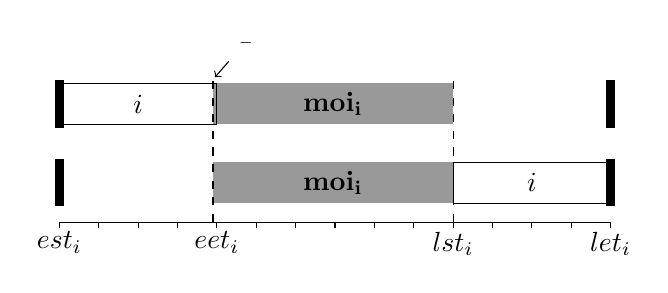
\begin{tikzpicture}
      [xscale=0.5, yscale= 0.4,node distance=0.5cm][decoration={brace}]
      \node (sil) at (0,0) {} ;
      \node (sir) at (10,0) {}; 
      \draw (10,0) node[below] {$lst_i$};
      \node (eir) at (14,0) {} ;
      \node (eil) at (4,0) {} ;
      \draw (4,0) node [below]  {$eet_i$} ;
      \draw (sil.center) node[below] {$est_i$}--
      (eir.center) node[below] {$let_i$};
      
      \draw[<-] (3.95, 4.6) -- (4.3,5.1) node[above=0.2cm,right] {\scriptsize $\EE^{-}$};
      \draw[line width=3pt] (0,0.5) -- (0,2);
      \draw[line width=3pt] (14,0.5) -- (14,2);
      \draw[line width=3pt] (0,3) -- (0,4.5);
      \draw[line width=3pt] (14,3) -- (14,4.5);

      \fill[gray!80] (3.9,0.6) rectangle (10,1.9) node[midway,color=black] {$\mathbf{moi_i}$};
      \fill[gray!80] (3.9,3.1) rectangle (10,4.4) node[midway,color=black] {$\mathbf{moi_i}$};
      
      \draw (0,3.1) rectangle (4,4.4) node[midway] {$i$};
      \draw (10,0.6) rectangle (14,1.9) node[midway] {$i$};

      \draw[dashed] (3.9,0) -- (3.9,4.5);
      \draw[dashed] (10,0) -- (10,4.5);

      \foreach \i in {0,...,14} {
        \draw (\i,0)  -- (\i,-0.2);
      }
    \end{tikzpicture}
  \end{center}

  \caption{Intervalle minimum de superposition d'une activité}
  \label{fig:moi_CECSP}
\end{figure}
\end{ex}

La notion d'intervalle minimum de superposition permet, dans un
premier temps, d'améliorer le raisonnement disjonctif. En effet, dans
le cas où deux activités $i$ et $j$ ne peuvent être exécutée en
parallèle, la fenêtre de temps de $j$ ne peut contenir un point de
temps que $i$ devra forcément chevaucher, i.e. contenu dans
$moi_i$. Ceci nous permet de définir la règle d'ajustement suivante:  

\begin{reg}
\label{reg:RDR_CECSP}
  Soient deux activités $i$ et $j$ telles que $i$ ne possède pas de
  partie obligatoire et que $\bmin + \bmin[j] > R$. Si ordonnancer l'activité
 $j$ à sa date de début au plus tôt la fait se superposer complètement
 à l’intervalle minimal de superposition de $i$ ($moi_i \subseteq
 [\ES[j],\EE[j]{]}$), alors $\ES[j] \ge \EE$.
\end{reg}

\begin{ex}
Considérons les deux activités suivantes: 
\begin{center}
\begin{tabular}{|P{1cm}|P{1cm}P{1cm}P{1cm}P{1cm}P{1cm}P{2cm}|}
    \hline
    act & \ES & \LE & W_i & \bmin & \bmax & f_i(b_i(t))  \\
    \hline
   i & 0 & 14 & 28 & 2 & 3 & 2*b_i(t) +1\\
   j & 2 & 20 & 49 & 2 & 4 & voir fig~\ref{fig:fonct_ CECSP}\\
    \hline
  \end{tabular}
\end{center}


La règle~\ref{reg:RDR_CECSP} est illustrée par la
figure~\ref{fig:RDR_CECSP}. Dans les figures~\ref{fig:RDR_CECSPa} et~\ref{fig:RDR_CECSPb}, on
peut constater que si l'activité $j$
commence à $\ES[j]$, alors elle intersecterait complètement $moi_i$ et
il serait impossible d'ordonnancer $i$. Sur la figure~\ref{fig:RDR_CECSPc}, $\ES[j]$ a été ajusté et l'activité $j$ ne peut commencer
avant  $t > \min{moi_i}$.
  \begin{figure}[htb!] 
    \subcaptionbox{Si $j$ commence au temps $2$...\label{fig:RDR_CECSPa}}[0.45\linewidth]{
    \centering
    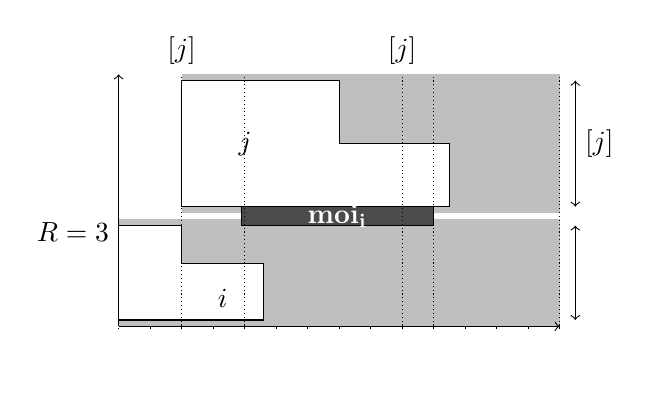
\begin{tikzpicture} [yscale=0.4,xscale=0.4]   
        \node (O) at (0,0) {};
      \foreach \i in {1,...,14} {
        \draw (\i,0) -- (\i,-0.1) ;
      }
      \fill[gray!50] (0,0) rectangle (14,3.4);
      \fill[gray!50] (2,3.6) rectangle (14,8);
      
      \draw[fill=white] (0,0.2) -- (0,3.2)   -- (2,3.2) -- (2,2) --node[midway,below=0.2cm] {$i$}
      (4.6,2) -- (4.6,0.2) -- cycle;
      
      \draw[fill=white] (2,3.8) -- (2,7.8)  node[midway,right=0.6cm] {$j$} -- (7,7.8) -- (7,5.8) --
      (10.5,5.8) -- (10.5,3.8) -- cycle;

        \draw[fill=black!70!] (3.9,3.2) rectangle
        (10,3.8) node[midway,white] {$\mathbf{moi_i}$};

      \draw[->] (0,0) -- (14,0);
      \draw[->] (0,0) -- (0,8) ;
      \draw (0,3) node[left] {$R=3$};
      \draw[densely dotted] (2,-0.1) -- (2,8) node[above] {$\ES[j]$};
      \draw[densely dotted] (9,-0.1) -- (9,8) node[above] {$\EE[j]$};
      \draw[densely dotted] (0,-0.1)  node[below] {$\ES$}-- (0,8);
      \draw[densely dotted] (4,-0.1 ) node[below=0.4cm] {$\EE$}-- (4,8) ;
      \draw[densely dotted] (10,-0.1) node[below] {$\LS$} -- (10,8) ;
      \draw[densely dotted] (14,-0.1) node[below right] {$\LE$} -- (14,8) ;
      \draw[<->] (14.5,0.2) -- (14.5,3.2) node[midway,right] {$\bmax$} ;
      \draw[<->] (14.5,3.8) -- (14.5,7.8) node[midway,right] {$\bmax[j]$} ;   
    \end{tikzpicture}
  }
    \subcaptionbox{...alors $j$ chevauche forcément $moi_i$\label{fig:RDR_CECSPb}}[0.45\linewidth]{
        \centering
        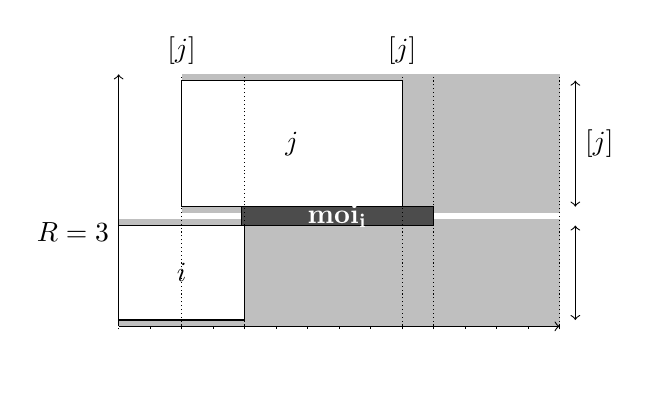
\begin{tikzpicture}[yscale=0.4,xscale=0.4]
      \node (O) at (0,0) {};
      \foreach \i in {1,...,14} {
        \draw (\i,0) -- (\i,-0.1) ;
      }
      \fill[gray!50] (0,0) rectangle (14,3.4);
      \fill[gray!50] (2,3.6) rectangle (14,8);
      
      \draw[fill=white] (0,0.2) rectangle (4,3.2) node[midway]
      {$i$};
      \draw[fill=white] (2,3.8) rectangle (9,7.8) node[midway]
      {$j$}; 
      \draw[fill=black!70!] (3.9,3.2) rectangle
        (10,3.8) node[midway,white] {$\mathbf{moi_i}$};

      
      \draw[->] (0,0) -- (14,0);
      \draw[->] (0,0) -- (0,8) ;
      \draw (0,3) node[left] {$R=3$};
      \draw[densely dotted] (2,-0.1) -- (2,8) node[above] {$\ES[j]$};
      \draw[densely dotted] (9,-0.1) -- (9,8) node[above] {$\EE[j]$};
      \draw[densely dotted] (0,-0.1)  node[below] {$\ES$}-- (0,8);
      \draw[densely dotted] (4,-0.1 ) node[below=0.4cm] {$\EE$}-- (4,8) ;
      \draw[densely dotted] (10,-0.1) node[below] {$\LS$} -- (10,8) ;
      \draw[densely dotted] (14,-0.1) node[below right] {$\LE$} -- (14,8) ;
      % \draw[densely dotted] (6,-0.1) -- (6,8) node[above] {$\ES[j]^{'}$};
      % \draw[->] (1.8,5.8) -- (5.2,5.8);
      \draw[<->] (14.5,0.2) -- (14.5,3.2) node[midway,right] {$\bmax$} ;
      \draw[<->] (14.5,3.8) -- (14.5,7.8) node[midway,right]
      {$\bmax[j]$} ;
    \end{tikzpicture}
   }
    \subcaptionbox{$\ES[j]$ peut être ajusté\label{fig:disj_CECSPc}}[\linewidth]{    \centering
      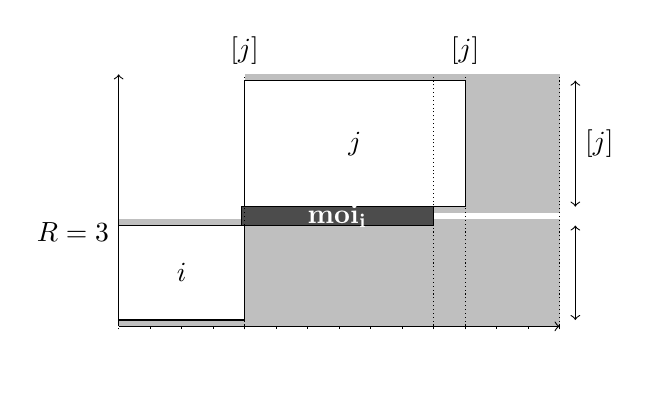
\begin{tikzpicture} [yscale=0.4,xscale=0.4]
      \node (O) at (0,0) {};
      \foreach \i in {1,...,14} {
        \draw (\i,0) -- (\i,-0.1);
      }
      \fill[gray!50] (0,0) rectangle (14,3.4);
      \fill[gray!50] (4,3.6) rectangle (14,8);
      
      \draw[fill=white] (0,0.2) rectangle (4,3.2) node[midway]
      {$i$};
      \draw[fill=white] (4,3.8) rectangle (11,7.8) node[midway]
      {$j$};
      \draw[fill=black!70!] (3.9,3.2) rectangle
        (10,3.8) node[midway,white] {$\mathbf{moi_i}$};

      \draw[->] (0,0) -- (14,0);
      \draw[->] (0,0) -- (0,8) ;
      \draw (0,3) node[left] {$R=3$};
      \draw[densely dotted] (4,-0.1) -- (4,8) node[above] {$\ES[j]$};
      \draw[densely dotted] (11,-0.1) -- (11,8) node[above] {$\EE[j]$};
      \draw[densely dotted] (0,-0.1)  node[below] {$\ES$}-- (0,8);
      \draw[densely dotted] (4,-0.1 ) node[below=0.4cm] {$\EE$}-- (4,8) ;
      \draw[densely dotted] (10,-0.1) node[below] {$\LS$} -- (10,8) ;
      \draw[densely dotted] (14,-0.1) node[below right] {$\LE$} --
      (14,8) ;
      \draw[<->] (14.5,0.2) -- (14.5,3.2) node[midway,right] {$\bmax$} ;
      \draw[<->] (14.5,3.8) -- (14.5,7.8) node[midway,right] {$\bmax[j]$} ;

  \end{tikzpicture}
}
  \caption{Raisonnement disjonctif restreint pour le \CECSP.}
  \label{fig:disj_CECSP}
\end{figure}
\end{ex}

La règle~\ref{reg:RDR_CUSP} compare seulement les consommations de $i$
et de $j$ avec la capacité de la ressource $R$. Cependant, les
consommations obligatoires des autres activités peuvent ne pas laisser
$R$ unités de ressource durant l'intersection de $i$ et de $j$. La
règle suivante prend donc en considération le profil obligatoire de la
ressource. 

\begin{reg}
\label{reg:TTDR_CUSP}
Soient donc $i$ et $j$ deux activités qui ne possèdent pas de partie
obligatoire et telles que $ \bmin +\bmin[j] + \min_{t \in moi_i} TT_{\A}(t) >
R$.   Si ordonnancer l'activité
 $j$ à sa date de début au plus tôt la fait se superposer complètement
 à l’intervalle minimal de superposition de $i$ ($moi_i \subseteq
 [\ES[j],\EE[j]{]}$), alors $\ES[j] \ge \EE$.
\end{reg}

\begin{ex}
Considérons les deux activités suivantes: 
\begin{center}
\begin{tabular}{|P{1cm}|P{1cm}P{1cm}P{1cm}P{1cm}P{1cm}P{2cm}|}
    \hline
    act & \ES & \LE & W_i & \bmin & \bmax & f_i(b_i(t))  \\
    \hline
   i & 2 & 11 & 21 & 1 & 2 & 2*b_i(t) +1\\
   j & 1 & 20 & 14 & 1 & 2 & b_i(t)\\
   k & 2 & 11 & 18 & 2 & 2 & \frac{1}{3}b_i(t) + \frac{4}{3}\\
    \hline
  \end{tabular}
\end{center}


  Les activités $1$ et $2$ ne possèdent pas de partie obligatoire tandis
  que l'activité $3$ est forcément en cours d'exécution durant
  l'intervalle $[2,11[$. 


  \begin{figure}[!htb]
    \centering
    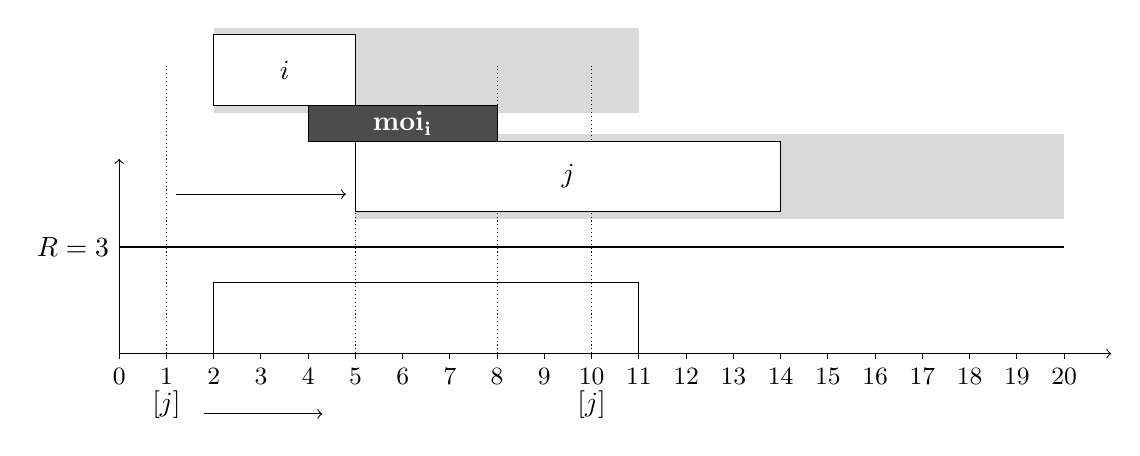
\begin{tikzpicture}
      [yscale=0.45,xscale=0.6]
      \node (O) at (0,0) {};
      \foreach \i in {0,1,...,20} {
        \draw (\i,0) -- (\i,-0.15) node[below] {\small $\i$};
      }
      
      \draw (2,0) rectangle (11,2);
      \fill[gray!30] (5,3.8) rectangle (20,6.2);
      \fill[gray!30] (2,6.8) rectangle (11,9.2);
      
      \draw [->] (1.2,4.5) -- (4.8,4.5);
      \draw [->] (1.8,-1.7) -- (4.3,-1.7);
      \draw[densely dotted] (1,-0.1) node[below=0.3cm] {$\ES[j]$}-- (1,8.2) ;
      \draw[densely dotted] (5,-0.1 ) node[below=0.3cm] {$\EE$}--
      (5,8.2);
      \draw[densely dotted] (10,-0.1) node[below=0.3cm] {$\EE[j]$} -- (10,8.2) ;
      \draw[densely dotted] (8,-0.1) node[below=0.3cm] {$\LS$} -- (8,8.2) ;
      
      \draw[fill=black!70!] (4,6) rectangle
      (8,7) node[midway,white] {$\mathbf{moi_i}$};
      
      \draw[fill=white] (2,7) rectangle (5,9) node[midway]
      {$i$};
      \draw[fill=white] (5,4) rectangle (14,6) node[midway]
      {$j$};
      
      \draw[->] (0,0) -- (21,0);
      \draw[->] (0,0) -- (0,5.5) ;
       \draw[thick] (0,3)  node[left] {$R=3$} -- (20,3);
       % \draw[densely dotted] (6,-0.1) -- (6,5.5) node[above] {$\ES[j]^{'}$};
      % \draw[->] (1.8,5.8) -- (5.2,5.8);  
    \end{tikzpicture}
    \caption{Illustration du Time-Tabe disjonctif}
    \label{fig:TTDR_CUSP}
  \end{figure}
L'intervalle $moi_i=[4,8]$ est complètement inclus dans l'intervalle
formé par $\ES[j]$ et $\EE[j]$, i.e. $[1,10[$. De plus, le minimum du
profil de consommation de la ressource dans $moi_i$ est de $2$. Donc,
les activités $i$ et $j$, consommant  au minimum  $1$ unité
de ressource, ne peuvent se chevaucher l'intervalle $[4,8]$. Donc
$\ES[j]$ peut être ajuster à $5$. 
\end{ex}

\subsection{Le Time-Table basé sur les flots}




\section{Algorithme de filtrage du raisonnement énergétique}
\label{sec:ER_CECSP}
\index{raisonnement énergétique!pour le CECSP}

Le paragraphe ci-dessous décrit l'adaptation du raisonnement
énergétique, introduit par~\cite{RELopez} pour la contrainte cumulative,
et décrit dans le paragraphe~\ref{sec:cumu_propag}. Nous commençons,
dans un premier temps par décrire l'algorithme de vérification de ce
raisonnement, puis nous présenterons les règles d'ajustements qui
peuvent être mises en place pour filtrer les domaines des
variables. Enfin, la dernière partie de ce paragraphe sera consacrée à
la caractérisation des intervalles d'intérêt pour l'algorithme de
vérification et pour les règles d'ajustement.

\subsection{Algorithme de vérification}

\subsubsection{Condition nécessaire d'existence de solution}
Pour décrire l'algorithme de vérification, nous rappelons d'abord
l'idée principale sur laquelle repose le raisonnement énergétique. Le
principe est donc, étant donné un intervalle $[t_1,t_2[$, de calculer
les consommations minimales de ressource des activités dans cette
intervalle et de les comparer à la quantité de ressource disponible
dans ce même intervalle. Si la ressource disponible n'est pas
suffisante pour ordonnancer les consommations minimales de toutes les
activités, une incohérence est détectée.

Dans le cas du \CUSP, la quantité de ressource requise par une
activité pouvait être calculée de manière directe. Ici, ce calcul sera
fait en deux fois: nous calculons d'abord la quantité d'énergie
requise par une activité à l'intérieur de l'intervalle $[t_1,t_2{[}$,
notée $\wb$, puis nous traduisons cette énergie en une quantité de
ressource, notée $\bb$. Ceci nous permettra ensuite de la comparer
avec la ressource disponible dans $[t_1,t_2{[}$.

Formellement ces quantités sont représentées par les expressions
suivantes: 
\begin{align}
  \wb= \min \int_{t_1}^{t_2} f_i(b_i(t))dt & & \text{sous 
\eqref{tw_CECSP}-\eqref{nrj_CECSP}}\\
  \bb= \min \int_{t_1}^{t_2} b_i(t)dt & & \text{sous 
\eqref{tw_CECSP}-\eqref{nrj_CECSP}}
\end{align}

Comme pour le cas du \CUSP, la fonction de marge, notée $SL(t_1,t_2)$,
permet de mesurer l'écart entre la quantité de ressource disponible et
les consommations minimales de toutes les tâches dans l'intervalle
${[}t_1,t_2{]}$. Cette fonction est définie de la manière suivante:
\[ SL(t_1,t_2)=B(t_2-t_1)-\sum\limits_{i \in A} \bb \]

Et ceci nous permet d'énoncer la condition nécessaire d'existence
d'une solution qui est à la base de l'algorithme de vérification du
raisonnement énergétique:

\begin{theo}
  \label{th:ER_CECSP}
  Soit $\I$ une instance du \CECSP. S'il existe $t_1 < t_2 \in
  \mathbb{R}^2$ tel que $SL(t_1,t_2) <0$ alors $\I$ ne peut pas avoir
  de solution.
\end{theo}

\begin{proof}
Par l'absurde, supposons qu'il existe $t_1 < t_2 \in \mathbb{R}^2$ tel
que $SL(t_1,t_2) > 0$ et que l'instance $\I$ soit satisfiable. Par
définition, $\bb$ est la quantité de ressource minimale que doit
consommer l'activité $i$ dans l'intervalle $[t_1,t_2{[}$. 

Donc, dans toute solution réalisable, nous avons: 
\begin{align*}
 & \int_{t_1}^{t_2} b_i(t)dt \ge \bb\\
\Rightarrow  & \sum_{i \in \A} \int_{t_1}^{t_2} b_i(t)dt \ge \sum_{i
               \in \A}  \bb > R(t_2-t_1)
\end{align*}
Et ceci contredit le fait que $\sum_{i \in \A} b_i(t) \le
R(t_2-t_1)$. 
\end{proof}

Dans un premier temps, nous allons nous intéressé au calcul de $\wb$,
le calcul de $\bb$ sera détaillé dans un second temps. 


\subsubsection{{\'E}nergie minimale dans un intervalle}

Pour calculer $\wb$, nous analysons les différentes configurations de
la consommation minimale d'une tâche. Remarquons que les
configurations conduisant à une consommation minimale dans
l'intervalle $[t_1,t_2{[}$ sont celles où l'activité est ordonnancée à
$\bmax$ à l'intérieur de cet intervalle. Ces configurations, décrites
dans la figure~\ref{fig:conso_CECSP}, peuvent être regroupée en trois
catégories:
\begin{itemize}
\item l'activité est {\it calée à
gauche} (figure~\ref{fig:conso_CECSPa}, \ref{fig:conso_CECSPb},
\ref{fig:conso_CECSPd} et \ref{fig:conso_CECSPg}): l'activité démarre
à $\ES$ et est ordonnancée à $\bmax$ pendant l'intervalle
$[\ES,t_1{[}$;
\item l'activité est {\it calée à
droite} (figure~\ref{fig:conso_CECSPb}, \ref{fig:conso_CECSPc},
\ref{fig:conso_CECSPf} et \ref{fig:conso_CECSPi}): l'activité finit à
$\LE$ et est ordonnancée à $\bmax$ pendant l'intervalle $[t_2,\LE{[}$;
\item l'activité est {\it centrée} (figure~\ref{fig:conso_CECSPe} et
\ref{fig:conso_CECSPh}): l'activité occupe tout l'intervalle
$[t_1,t_2[$, soit en étant ordonnancée à $\bmax$ pendant l'intervalle
$[\ES,t_1{[} \cup [t_2,\LE{[}$, soit en étant ordonnancée à $\bmin$
durant tout l'intervalle $[t_1,t_2{[}$.
\end{itemize}
En effet, lorsque l'activité est ordonnancée à $\bmax$ pendant
l'intervalle $[\ES,t_1{[} \cup [t_2,\LE{[}$, il peut arriver que la
quantité d'énergie restant à apporter à l'activité durant l'intervalle
$[t_1,t_2[$ ne soit pas suffisante pour assurer la satisfaction de la
contrainte de consommation minimale~\eqref{req_CECSP}. Le cas où
l'activité est ordonnancée à $\bmin$ durant tout l'intervalle
$[t_1,t_2{[}$ doit donc être considéré.

\begin{figure}[!htb]  
\centering
\subcaptionbox{\label{fig:conso_CECSPa}}[0.3\linewidth]{
  \begin{tikzpicture}
    [xscale=0.37,yscale=0.3]
    \node[] (O) at (0,0) {};
    \node[label={[shift={(-0.4,-0.4)}]$\bmin$}] (bmin) at (0,1) {};
    \node[label={[shift={(-0.4,-0.4)}]$\bmax$}] (bmax) at (0,4) {};
    \node (t1) at (6,0) {}; 
    \node[label={[shift={(0,-0.8)}]$\ES$}] (ri) at (1,0) {};
    \node (t2) at (7,0) {};

    \draw[->] (O.center) -- (8,0)node[below] {$t$};
    \draw (O.south) -- (bmax.north);
    \draw (bmin.center) -- (8,1);
    \draw (bmax.center) -- (8,4);
    \draw(ri.south) -- (ri.center);
    \draw[fill=white] (ri.center) rectangle (5,4);
    \draw[pattern=north west lines] (ri.center) rectangle (5,4);
    \draw[thick] (t1.south) -- (6,4.1) node[above] {$t_1$};
    \draw[thick] (t2.south) -- (7,4.1) node[above] {$t_2$};
  \end{tikzpicture}}
\hfill
\subcaptionbox{\label{fig:conso_CECSPb}}[0.3\linewidth]{
  \begin{tikzpicture}
    [xscale=0.37,yscale=0.3]
    \node[] (O) at (0,0) {};
    \node[label={[shift={(-0.4,-0.4)}]$\bmin$}] (bmin) at (0,1) {};
    \node[label={[shift={(-0.4,-0.4)}]$\bmax$}] (bmax) at (0,4) {};
    \node (t1) at (1,0) {}; 
    \node[label={[shift={(0,-0.8)}]$\ES$}] (ri) at (2,0) {};
    \node (t2) at (7,0) {};
    \node[label={[shift={(0,-0.8)}]$\LE$}] (di) at (6,0) {};

    \draw[->] (O.center) -- (8,0)node[below] {$t$};
    \draw (O.south) -- (bmax.north);
    \draw (bmin.center) -- (8,1);
    \draw (bmax.center) -- (8,4);
    \draw(ri.south) -- (ri.center);
    \draw(di.south) -- (di.center);
    \draw[fill=white] (2.5,0) rectangle (5.5,4);
    \draw[pattern=north west lines] (2.5,0) rectangle (5.5,4);
    \draw[thick] (t1.south) -- (1,4.1) node[above] {$t_1$};
    \draw[thick] (t2.south) -- (7,4.1) node[above] {$t_2$};
  \end{tikzpicture}}
\hfill
\subcaptionbox{\label{fig:conso_CECSPc}}[0.3\linewidth]{
  \begin{tikzpicture}
    [xscale=0.37,yscale=0.3]
    \node[] (O) at (0,0) {};
    \node[label={[shift={(-0.4,-0.4)}]$\bmin$}] (bmin) at (0,1) {};
    \node[label={[shift={(-0.4,-0.4)}]$\bmax$}] (bmax) at (0,4) {};
    \node (t1) at (0.5,0) {};
    \node (t2) at (1.5,0) {};
    \node[label={[shift={(0,-0.8)}]$\LE$}] (di) at (7,0) {};
    
    \draw[->] (O.center) -- (8,0)node[below] {$t$};
    \draw (O.south) -- (bmax.north);
    \draw (bmin.center) -- (8,1);
    \draw (bmax.center) -- (8,4);
    \draw[fill=white] (3,0) rectangle (7,4);
    \draw[pattern=north west lines] (3,0) rectangle (7,4);
    \draw(di.south) -- (di.center);
    \draw[thick] (t1.south) -- (0.5,4.1) node[above] {$t_1$};
    \draw[thick] (t2.south) -- (1.5,4.1) node[above] {$t_2$};
  \end{tikzpicture}}


\subcaptionbox{\label{fig:conso_CECSPd}}[0.3\linewidth]{
\begin{tikzpicture}
  [xscale=0.37,yscale=0.3]
    \node[] (O) at (0,0) {};
    \node[label={[shift={(-0.4,-0.4)}]$\bmin$}] (bmin) at (0,1) {};
    \node[label={[shift={(-0.4,-0.4)}]$\bmax$}] (bmax) at (0,4) {};
    \node (t1) at (4,0) {};
    \node (t2) at (7,0) {};
    \node[label={[shift={(0,-0.8)}]$\LE$}] (di) at (6,0) {};
    \node[label={[shift={(0,-0.8)}]$\ES$}] (ri) at (1,0) {};
    
    \draw[->] (O.center) -- (8,0)node[below] {$t$};
    \draw (O.south) -- (bmax.north);
    \draw (bmin.center) -- (8,1);
    \draw (bmax.center) -- (8,4);
    \draw[fill=white] (ri.center) rectangle (4,4);
    \draw[pattern=north west lines] (ri.center) rectangle (4,4);
    \draw[fill=white] (t1.center) rectangle (5,1.5);
    \draw[pattern=north west lines] (t1.center) rectangle (5,1.5);
    \draw(di.south) -- (di.center);
    \draw(ri.south) -- (ri.center);
    \draw[thick] (t1.south) -- (4,4.1) node[above] {$t_1$};
    \draw[thick] (t2.south) -- (7,4.1) node[above] {$t_2$};
  \end{tikzpicture}}
\hfill
\subcaptionbox{\label{fig:conso_CECSPe}}[0.3\linewidth]{
\begin{tikzpicture}
 [xscale=0.37,yscale=0.3]
 \node[] (O) at (0,0) {};
 \node[label={[shift={(-0.4,-0.4)}]$\bmin$}] (bmin) at (0,1) {};
 \node[label={[shift={(-0.4,-0.4)}]$\bmax$}] (bmax) at (0,4) {};
 \node (t1) at (2.5,0) {}; 
 \node[label={[shift={(0,-0.8)}]$\ES$}] (ri) at (1.5,0) {};
 \node (t2) at (6,0) {};
 \node[label={[shift={(0,-0.8)}]$\LE$}] (di) at (7,0) {};
 
  \draw[->] (O.center) -- (8,0)node[below] {$t$};
  \draw (O.south) -- (bmax.north);
  \draw (bmin.center) -- (8,1);
  \draw (bmax.center) -- (8,4);
  \draw(ri.south) -- (ri.center);
  \draw(di.south) -- (di.center);
  \draw[fill=white] (2.5,0) rectangle (1.5,4);
  \draw[pattern=north west lines] (2.5,0) rectangle (1.5,4);
  \draw[fill=white] (2.5,0) rectangle (6,2);
  \draw[pattern=north west lines] (2.5,0) rectangle (6,2);
  \draw[fill=white] (6,0) rectangle (7,4);
  \draw[pattern=north west lines] (6,0) rectangle (7,4);
  \draw[thick] (t1.south) -- (2.5,4.1) node[above] {$t_1$};
  \draw[thick] (t2.south) -- (6,4.1) node[above] {$t_2$};
 \end{tikzpicture}}
\hfill
\subcaptionbox{\label{fig:conso_CECSPf}}[0.3\linewidth]{
  \begin{tikzpicture}
 [xscale=0.37,yscale=0.3]
 \node[] (O) at (0,0) {};
 \node[label={[shift={(-0.4,-0.4)}]$\bmin$}] (bmin) at (0,1) {};
 \node[label={[shift={(-0.4,-0.4)}]$\bmax$}] (bmax) at (0,4) {};
 \node[label={[shift={(0,-0.8)}]$\LE$}] (di) at (7,0) {};
 \node (t1) at (1,0) {}; 
 \node[label={[shift={(0,-0.8)}]$\ES$}] (ri) at (2.5,0) {};
 \node (t2) at (4,0) {};
 
 \draw[->] (O.center) -- (8,0)node[below] {$t$};
 \draw (O.south) -- (bmax.north);
 \draw (bmin.center) -- (8,1);
 \draw (bmax.center) -- (8,4);
 \draw(di.south) -- (di.center);
 \draw(ri.south) -- (ri.center);
 \draw[fill=white] (t2.center) rectangle (7,4);
 \draw[pattern=north west lines] (t2.center) rectangle (7,4);
 \draw[fill=white] (t2.center) rectangle (3.2,2);
 \draw[pattern=north west lines] (t2.center) rectangle (3.2,2);
 \draw[thick] (t1.south) -- (1,4.1) node[above] {$t_1$};
 \draw[thick] (t2.south) -- (4,4.1) node[above] {$t_2$};
 \end{tikzpicture}}



\subcaptionbox{\label{fig:conso_CECSPg}}[0.3\linewidth]{
  \begin{tikzpicture}
  [xscale=0.37,yscale=0.3]
    \node[] (O) at (0,0) {};
    \node[label={[shift={(-0.4,-0.4)}]$\bmin$}] (bmin) at (0,1) {};
    \node[label={[shift={(-0.4,-0.4)}]$\bmax$}] (bmax) at (0,4) {};
    \node (t1) at (3,0) {};
    \node (t2) at (5,0) {};
    \node[label={[shift={(0,-0.8)}]$\LE$}] (di) at (7,0) {};
    \node[label={[shift={(0,-0.8)}]$\ES$}] (ri) at (1,0) {};
    
    \draw[->] (O.center) -- (8,0)node[below] {$t$};
    \draw (O.south) -- (bmax.north);
    \draw (bmin.center) -- (8,1);
    \draw (bmax.center) -- (8,4);
    \draw[fill=white] (t1.center) rectangle (1,4);
    \draw[pattern=north west lines] (t1.center) rectangle (1,4);
    \draw[fill=white] (t1.center) rectangle (3.7,1);
    \draw[pattern=north west lines] (t1.center) rectangle (3.7,1);
    \draw(di.south) -- (di.center);
    \draw(ri.south) -- (ri.center);
    \draw[thick] (t1.south) -- (3,4.1) node[above] {$t_1$};
    \draw[thick] (t2.south) -- (5,4.1) node[above] {$t_2$};
  \end{tikzpicture}}
\hfill
\subcaptionbox{\label{fig:conso_CECSPh}}[0.3\linewidth]{
  \begin{tikzpicture}
  [xscale=0.37,yscale=0.3]
   \node[] (O) at (0,0) {};
    \node[label={[shift={(-0.4,-0.4)}]$\bmin$}] (bmin) at (0,1) {};
    \node[label={[shift={(-0.4,-0.4)}]$\bmax$}] (bmax) at (0,4) {};
    \node (t1) at (2.5,0) {}; 
    \node[label={[shift={(0,-0.8)}]$\ES$}] (ri) at (1.5,0) {};
    \node (t2) at (6,0) {};
    \node[label={[shift={(0,-0.8)}]$\LE$}] (di) at (7,0) {};

    \draw[->] (O.center) -- (8,0)node[below] {$t$};
    \draw (O.south) -- (bmax.north);
    \draw (bmin.center) -- (8,1);
    \draw (bmax.center) -- (8,4);
    \draw(ri.south) -- (ri.center);
    \draw(di.south) -- (di.center);
    \draw[fill=white] (2.5,0) rectangle (2,2.7);
    \draw[pattern=north west lines] (2.5,0) rectangle (2,2.7);
    \draw[fill=white] (2.5,0) rectangle (6,1);
    \draw[pattern=north west lines] (2.5,0) rectangle (6,1);
    \draw[fill=white] (6,0) rectangle (7,4);
    \draw[pattern=north west lines] (6,0) rectangle (7,3);
    \draw[thick] (t1.south) -- (2.5,4.1) node[above] {$t_1$};
    \draw[thick] (t2.south) -- (6,4.1) node[above] {$t_2$};
  \end{tikzpicture}}
\hfill
\subcaptionbox{\label{fig:conso_CECSPi}}[0.3\linewidth]{
\begin{tikzpicture}
 [xscale=0.37,yscale=0.3]
 \node[] (O) at (0,0) {};
 \node[label={[shift={(-0.4,-0.4)}]$\bmin$}] (bmin) at (0,1) {};
 \node[label={[shift={(-0.4,-0.4)}]$\bmax$}] (bmax) at (0,4) {};
 \node[label={[shift={(0,-0.8)}]$\LE$}] (di) at (7,0) {};
 \node (t1) at (2.5,0) {}; 
 \node (t2) at (4,0) {};
 \node[label={[shift={(0,-0.8)}]$\ES$}] (ri) at (1,0) {};
 
 \draw[->] (O.center) -- (8,0)node[below] {$t$};
 \draw (O.south) -- (bmax.north);
 \draw (bmin.center) -- (8,1);
 \draw (bmax.center) -- (8,4);
 \draw(di.south) -- (di.center);
 \draw(ri.south) -- (ri.center);
 \draw[fill=white] (t2.center) rectangle (7,4);
 \draw[pattern=north west lines] (t2.center) rectangle (7,4);
 \draw[fill=white] (t2.center) rectangle (3.2,1);
 \draw[pattern=north west lines] (t2.center) rectangle (3.2,1);
 \draw[thick] (t1.south) -- (2.5,4.1) node[above] {$t_1$};
 \draw[thick] (t2.south) -- (4,4.1) node[above] {$t_2$}; 
 \end{tikzpicture}}
\caption{Les différentes configurations menant à une consommation minimale}
\label{fig:conso_CECSP}
\end{figure}
	
Il est facile de calculer l'expression de la consommation minimale
d'énergie dans un intervalle pour une fonction $f_i$ croissante. En
effet, les différentes configurations possibles étant toujours celle
où la tâche est exécutée à son rendement maximum en dehors de
l'intervalle ${[}t_1,t_2{[}$, il suffit de retrancher à $W_i$
l'énergie produite par l'exécution de la tâche en dehors de
${[}t_1,t_2{]}$. Il existe une exception à cette règle, produite par
la contrainte du rendement minimal, mais ce cas est facilement traiter
puisque l'énergie minimale correspond alors à la configuration où la
tâche est exécutée à son rendement minimal durant ${[}t_1,t_2{[}$. 

Pour donner l'expression mathématique de $\wb$ , nous introduisons
trois notations. $\wbLS$ (respectivement $\wbRS$ et $\wbCS$)
correspond à la quantité d'énergie apportée à l'activité $i$ dans
l'intervalle $[t_1,t_2[$ quand l'activité est calée à gauche
(respectivement calée à droite et centrée). Formellement, ces trois
quantités peuvent être exprimer de la manière suivante:
\begin{align}
\wbLS&= \max\left(0\, ,\, W_i- f_i(\bmax)\max(0,t_1 -
\ES)\right) \label{eq:LSnrj_CECSP}\\
\wbRS&= \max\left(0\, ,\, W_i- f_i(\bmax)\max(0,
\LE-t_2)\right)\label{eq:RSnrj_CECSP}\\
\wbCS&=\max\left( f_i(\bmin) * (t_2-t_1)\, ,\, W_i - f_i(\bmax)\max(0,
d_i - r_ i - t_2 + t_1) \right)\label{eq:CSnrj_CECSP}
\end{align}
Alors, l'expression de l'énergie minimale est le minimum de ces trois
quantités, i.e.
\begin{equation}
\wb=\min\left(\, \wbLS\, ,\,\wbRS\, ,\,\wbCS \, \right)
\end{equation} 

Nous allons maintenant utiliser l'expression de $\wb$ et la fonction
$f_i$ pour calculer $\bb$.

\subsubsection{Consommation minimale de la ressource}
	
Pour calculer l'expression de $\bb$, nous allons utiliser les
propriétés de la fonction $f_i$. En effet, une fois que nous avons
calculer $\wb$, nous voulons savoir quelle est la quantité minimale de
ressource que nous devons fournir à la tâche pour obtenir cette
quantité d'énergie dans l'intervalle ${[}t_1,t_2{[}$. Dans le cas où
la fonction $f_i$ est l'identité, nous avons que: $\bb=\wb$. Dans les
deux autres cas, i.e. $f_i$ est affine et $f_i$ est concave et affine
par morceaux, soit $I=[t_1,t_2[ \cap [\ES,\LE{[}$, alors trouver $\bb$
revient à résoudre le programme suivant:
\begin{align}
  \text{minimiser }   & \int_{I} b_i(t)dt \label{eq:conv_obj} \\
  \text{sous } & \int_{I} f_i(b_i(t))dt \ge \wb \label{eq:conv_nrj}\\
                     & \bmin \le b_i(t) \le \bmax \label{eq:conv_min}
\end{align}
En effet, l'objectif de ce programme est de minimiser la quantité de
ressource consommée dans l'intervalle $[t_1,t_2[$
(équation~\eqref{eq:conv_obj}), tout en s'assurant que l'énergie
requise, i.e. $\wb$, est bien apportée à l'activité
(équation~\eqref{eq:conv_nrj}). 

Nous utilisons ensuite le lemme~\ref{lemmaEn} pour simplifier ce
programme. En effet, le lemme affirme que, si $f_i$ est affine ou
concave et affine par morceaux, alors si une solution optimale
$b_i(t)$ pour le programme ci-dessus, cette solution peut être
transformée en une autre solution optimale vérifiant la propriété que
$b_i(t)$ soit constante et inférieure ou égale à
$\frac{\int_{I}b_i(t)dt}{|I|}$. Nous noterons $b_i$ cette
constante. Le programme simplifié s'écrit de la manière suivante:
\begin{align}
  \text{minimiser }   & b_i|I| \label{eq:convSimp_obj} \\
  \text{sous } & f_i(b_i)|I| \ge \wb \label{eq:convSimp_nrj}\\
                     &\bmin \le  b_i \le \bmax \label{eq:convSimp_nrj}
\end{align}


Ce programme peut être réécrit de la façon suivante: 
\[ b_i=\min\left( b \in [\bmin,\bmax]\ |\ f_i(b) \ge
    \frac{\wb}{|I|}\right)
\]

Nous pouvons remarquer que, si l'on suppose que $f_i(\bmax) (\LE - \ES
) \ge W_i$, nous sommes sûrs que la solution optimale vérifie $b_i \le
\bmax$. En effet, ceci est dû au fait qu'exécuter l'activité à une
faible consommation de ressource a un meilleur rendement que son
exécution à un rendement plus élevé, i.e. la fonction
$\frac{f_i(b_i(t))}{b_i(t)}$ est décroissante. 

De ce fait, seule la borne inférieure sur $b_i$, $\bmin$, doit être
considérée. Or, pour apporter l'énergie $\wb$ à l'activité dans
l'intervalle $I$, sa consommation $b_i$ doit vérifiée $f_i(b_i) \ge
\frac{\wb}{|I|}$ et donc $b_i \ge
f_i^{-1}\left(\frac{\wb}{|I|}\right)$. En couplant cette contrainte
avec la contrainte de consommation minimale, nous obtenons, si $\bmin
\neq 0$:
\[
 b_i= \max\left(\, \bmin \, ,\, 
    f_i^{-1}\left(\frac{\wb}{|I|}\right)\, \right)
\]
Et si $\bmin = 0$, nous avons:
\[
 b_i=  f_i^{-1}\left(\frac{\wb}{|I|}\right)
\]
Nous allons maintenant donner l'expression de $\bb$  en fonction des
coefficients $a_{ip}$  et $c_{ip}$ de la fonction $f_i$. Pour
simplifier la compréhension, nous commençons par détailler cette
expression dans le cas où $f_i$ est affine puis nous la généraliserons
dans le cas où $f_i$ est concave et affine par morceaux. 

\paragraph{Fonctions affines}

Dans ce paragraphe, nous allons décrire l'expression de $\bb$ dans le
cas où la fonction $f_i$ est affine, i.e. de la forme $a_ib+c_i$. Dans
ce cas-là, nous avons:  
\[f_i^{-1}\left( \frac{\wb}{|I|}\right)= \frac{ \wb- c_i|I|}{a_i|I|}
\]
Et donc, si $\bmin\neq 0$: 
\begin{equation}
\bb= \max\left(b_i^{min} \frac{\wb}{f_i(b_i^{min})} \, ,\,  
  \frac{1}{a_i}\left(\wb-|I|c_{i})\right)\right)
\end{equation}
Et si $\bmin=0$: 
\[
\bb=  \frac{1}{a_i}\left(\wb-|I|c_{i})\right)
\]
Notons que, le premier cas correspond au cas où l'intervalle $I$ est
suffisamment grand pour ordonnancer l'activité $i$ à $\bmin$ et lui
apporter l'énergie requise, i.e. $\wb$. En effet, comme ordonnancer
$i$ à $\bmin$ a la meilleur rendement, si l'on peut, i.e. l'intervalle
est assez grand, c'est cette valeur que l'on va choisir pour
$b_i$. Si, au contraire, l'intervalle n'est pas suffisamment grand,
c'est $f_i^{-1}(\wb/|I|) \times |I|$ que l'on va choisir. Ceci est
détaillé dans l'exemple~\ref{ex:convLin_CECSP}.

\begin{ex}
\label{ex:convLin_CECSP}

\end{ex}

Ce raisonnement peut être étendu dans le cas où $f_i$ est concave et
affine par morceaux. 

\paragraph{Fonctions concave et affine par morceaux}

Dans le cas des fonctions concaves et affines par morceaux, le
raisonnement décrit au paragraphe précédent peut être généralisé. En
effet, comme dans le cas des fonctions affines, la fonction de
rendement, $f_i(b_i(t))/b_i(t)$, est décroissante. Donc, il est
toujours préférable d'exécuter l'activité avec une consommation de
ressource aussi basse que possible. La condition selon laquelle on
peut ou non exécuter l'activité $i$ avec une consommation $b_i$ dépend
donc de la taille de l'intervalle $I$. 

Si $\bmin\neq 0$ et si l'intervalle est suffisamment grand, on va donc
exécuter l'activité à $\bmin$. Sinon, et si l'intervalle est
suffisamment grand, nous essayons d'exécuter l'activité avec une
consommation $b_i \in ]\bmin,x_2^i]$, etc. Dans le cas où $\bmin \neq
0$, l'expression de $\bb$ est formalisée ci-dessous:
\[f_i^{-1}\left(\frac{\wb}{|I|}\right)=\left\{
\begin{aligned}
\bmin & \qquad & \text{si } |I| \ge \frac{\wb}{f_i(\bmin)}\\
\frac{\wb -c_{i1}|I|}{a_{i1}|I|} & \qquad & \text{si } \frac{\wb}{f_i(\bmin)}
> |I| > \frac{\wb}{f_i(x^i_2)} \\
\frac{\wb -c_{i2}|I|}{a_{i2}|I|} & \qquad & \text{si }  \frac{\wb}{f_i(x^i_2)}
\ge |I| > \frac{\wb}{f_i(x^i_3)}\\
 & \qquad \vdots& \\
\frac{\wb -c_{iP_i}|I|}{a_{iP_i}|I|} & \qquad & \text{si }  \frac{\wb}{f_i(x^i_{P_i}}
\ge |I| > \frac{\wb}{f_i(\bmax)}\end{aligned}
\right.
\]
Et ceci, nous donne l'expression de $\bb$ suivante:
\begin{equation}
\bb= 
  \max \left\{b_i^{min} \frac{\wb}{f_i(b_i^{min})},
  \max_{ p \in \P_i} \left(\frac{1}{a_{ip}}(\wb-|I|c_{ip})\right)\right\}
\end{equation}
Dans le cas où $\bmin=0$, nous avons: 
\[
\bb= 
  \max_{ p \in \P_i} \left(\frac{1}{a_{ip}}(\wb-|I|c_{ip})\right)
\]
Un exemple du calcul de $\bb$ dans le cas d'une fonction $f_i$ concave
et linéaire par morceaux est décrit dans
l'exemple~\ref{ex:convPWL_CECSP}.

\begin{ex}
\label{ex:convPWL_CECSP}

\end{ex}

\subsection{Les ajustements de borne}
\label{sec:adjustment_tw}
 
Dans ce paragraphe nous décrivons les ajustements qui peuvent être
faits sur les fenêtre de temps des activités. Tout d'abord, nous
introduisons les notations suivantes: $\bbLS$ (respectivement $\bbRS$
et $\bbCS$) correspond à la quantité de ressource consommée par
l'activité $i$ dans l'intervalle $[t_1,t_2[$ quand l'activité est
calée à gauche (respectivement calée à droite et
centrée). Formellement, ces trois quantités peuvent être exprimer de
la manière suivante:
\begin{align}
\bbLS&=   \max \left\{b_i^{min} \frac{\wbLS}{f_i(b_i^{min})},
  \max_{ p \in \P_i} \left(\frac{1}{a_{ip}}(\wbLS-|I|c_{ip})\right)\right\}\\
\bbRS&=   \max \left\{b_i^{min} \frac{\wbRS}{f_i(b_i^{min})},
  \max_{ p \in \P_i} \left(\frac{1}{a_{ip}}(\wbRS-|I|c_{ip})\right)\right\}\\
\bbCS&=  \max \left\{b_i^{min} \frac{\wbCS}{f_i(b_i^{min})},
  \max_{ p \in \P_i} \left(\frac{1}{a_{ip}}(\wbCS-|I|c_{ip})\right)\right\}
\end{align}

Nous allons décrire deux règles d'ajustements pour les fenêtres du
temps du \CECSP. La première permet d'ajuster $\LS$ et la seconde
$\ES$ et nous avons des ajustements symétriques pour $\EE$ et $\LE$. 

Pour les premier ajustements décrits, nous allons essayer de faire
démarrer l'activité après $t_1$et si la quantité de ressource
disponible n’est pas suffisante pour ordonnancer les consommations
minimales de toutes les activités – excepté celle de l’activité i qui
est remplacée par $\bbRS$ – alors, nous pouvons déduire que l’activité
doit commencer avant $t_1$.

\begin{reg}
\label{reg:ajust_CECSP}
S’il existe un intervalle $[t_1 , t_2 [$ avec $t_1 > \ES$ et une
activité $i$ pour lesquels:
\[ \sum_{\substack{j \in \A\\ j\neq i}} \bb[j] + \bbRS > R(t_2-t_1)
\]
alors, on a:
\[ \LS \le t_1 - \frac{1}{\bmax}\left(\sum_{\substack{j \in \A\\ j\neq i}} \bb[j] + \bbRS - R(t_2-t_1)\right)
\]
\end{reg}

\begin{proof}
Soit $i$ et $[t_1,t_2[$ vérifiant la condition de la
règle~\ref{reg:ajust_CECSP}. Supposons que l'activité $i$ démarre à
$t_1$. 

La consommation minimale de $i$ dans $[t_1,t_2[$ est donc $\bbRS$. On
a donc que $\sum_{\substack{j \in \A\\ j\neq i}} \bb[j] + \bbRS $ est
la consommation minimale de toutes les activités dans $[t_1,t_2[$
quand l'activité $i$ commence à $t_1$. Donc, si cette quantité est
plus grande que la quantité de ressource disponible dans l'intervalle
$[t_1,t_2[$, i.e. $R(t_2-t_1)$, on obtient une contradiction avec le
fait que l'instance soit réalisable et $i$ doit commencer avant
$t_1$. 

Pour calculer la nouvelle date de début au plus tard de $i$,
remarquons que la quantité de ressource devant être consommée avant
$t_1$ est d'au moins $\sum_{\substack{j \in \A\\ j\neq i}} \bb[j] +
\bbRS - R(t_2-t_1)$, i.e. ce qui ne ``rentrait'' pas dans
$[t_1,t_2[$. Comme nous cherchons une borne supérieure sur la date de
début de $i$, nous cherchons donc à ordonnancer cette partie de
l'activité le plus rapidement possible. 

Le temps minimal requis pour ordonnancer cette
consommation étant obtenu en exécutant l'activité à $\bmax$, nous
obtenons comme borne supérieure sur la date de début de $i$:
$1/\bmax \times \left(\sum_{\substack{j \in \A\\ j\neq
i}} \bb[j] + \bbRS - R(t_2-t_1)\right)$
\end{proof}

De manière similaire, nous avons les ajustements suivants sur la date
de début au plus tôt d'une activité. 
\begin{reg}
\label{ajustRi_CECSP}
S'il existe un intervalle $[t_1,t_2[$ avec $ t_2 > \LE$ et une
activité $i$ telle que $\bmin \neq 0$ pour lesquels:
  \[ \sum_{\substack{j \in \A \\ j \neq i}} \bb[j] +
    \min(\bbCS,\bbLS) > R (t_2-t_1)\] 
  alors
  \[ \ES \ge t_2 - \frac{1}{\bmin} \left(R (t_2-t_1) -\sum_{\substack{j
\in \A \\ j \neq i}} \bb[j] \right) \]
\end{reg}

\begin{proof}
Soit $i$ et $[t_1,t_2[$ vérifiant la condition de la
règle~\ref{reg:ajust_CECSP}. Nous allons décider si $i$ peut commencer
avant $t_1$. Les configurations où l'activité $i$ démarre avant $t_1$
et consomme le moins de ressource possible dans $[t_1,t_2[$ sont les
configurations où $i$ est soit calée à gauche, soit centrée.

La consommation minimale de $i$ dans l'intervalle $[t_1,t_2[$ quand
$i$ commence avant $t_1$ est donc $\min( \bbLS, \bbCS)$. On a donc que
$\sum_{\substack{j \in \A\\ j\neq i}} \bb[j] + \min( \bbLS, \bbCS) $
est la consommation minimale de toutes les activités dans $[t_1,t_2[$
quand l'activité $i$ commence avant $t_1$. Donc, si cette quantité est
plus grande que la quantité de ressource disponible dans l'intervalle
$[t_1,t_2[$, i.e. $R(t_2-t_1)$, on obtient une contradiction avec le
fait que l'instance soit réalisable et $i$ doit commencer après $t_1$.

Pour calculer la nouvelle date de début au plus tard de $i$,
remarquons que la quantité de ressource disponible dans $[t_1,t_2[$
pour exécuter $i$ est de $R(t_2-t_1) -\sum_{\substack{j \in \A\\
j\neq i}} \bb[j]$. Comme nous cherchons une borne inférieure sur la date de
début de $i$, nous cherchons donc à ordonnancer cette partie de
l'activité le moins rapidement possible. 

Le temps maximal requis pour ordonnancer cette consommation étant
obtenu en exécutant l'activité à $\bmin$, et, comme $\bmin \neq 0$,
l'activité ne peut être préemptée, nous savons que l'activité doit
être en cours à $t_2$. Nous obtenons alors comme borne inférieure sur
la date de début de $i$:
$t_2 - 1/\bmin \left(R (t_2-t_1) -\sum_{\substack{j
\in \A \\ j \neq i}} \bb[j] \right) $
\end{proof}

\begin{ex}
 Considérons l'instance à $3$ activités et avec $R=5$ suivante:

  \begin{center}
    \begin{tabular}{|P{1cm}|P{1cm}P{1cm}P{1cm}P{1cm}P{1cm}P{2cm}|} 
      \hline 
      act. & \ES & \LE & W_i & \bmin& \bmax & f_i(b_i(t))\\ 
      \hline 
      1 & 0 & 6 & 28 & 1 & 5 & 2b_i(t)+1\\ 
      2 & 2 & 6 & 32 & 2 & 5 & b_i(t)+5\\ 
      3 & 2 & 5 & 6 & 2 & 2 & b_i(t)\\ 
      \hline
    \end{tabular}
  \end{center}
Une solution réalisable est décrit par la figure~\ref{exSol}.
\begin{figure}[!htb]
  \begin{center} 
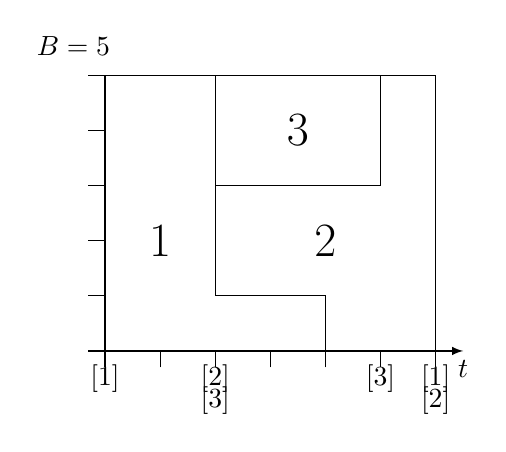
\begin{tikzpicture}
[scale=0.7]
\node (O) at (0,0) {};
\node (2) at (4,2) {\LARGE $2$};
\node (1) at (1,2) {\LARGE $1$};
\node (3) at (3.5,4) {\LARGE $3$};
\node[label={[shift={(-0.4,0)}]$B=5$}] (B) at (0,5) {};


\node (r1) at (0,-0.5) {$\ES[1]$}; 
\node (r2) at (2,-0.5) {$\ES[2]$};
\node (r3) at (2,-0.9) {$\ES[3]$};
\node (d1) at (6,-0.5) {$\LE[1]$};
\node (d2) at (6,-0.9) {$\LE[2]$};
\node (d3) at (5,-0.5) {$\LE[3]$};


\draw[->,>=latex] (6,0) -- (6.5,0) node[below] {$t$};

%\draw (0,0) rectangle (6,5);
\draw (4,0) -- (6,0) -- (6,5) -- (5,5);

   \draw (2,5) -- (2,1) -- (4,1) -- (4,0) -- (0,0) -- (0,5) -- cycle;

\draw (2,3) -- (5,3) -- (5,5) -- (2,5) ;


\foreach \i in {0,...,5}
{
  \draw (\i,-0.3) -- (\i,0);
  \draw (-0.3,\i) -- (0,\i);
}

 \draw (6,-0.3) -- (6,0);

\end{tikzpicture}
    \caption{Une solution réalisable du \CECSP}
    \label{exSol}
  \end{center}
\end{figure}

Nous allons ajuster la fenêtre de temps de l'activité $1$. Pour cela,
considérons l'intervalle $[t_1,t_2[=[2,5[$. On a:
\begin{itemize}
  \item $\bb[2][2][5]=7$
  \item $\bb[3][2][5]=6$
  \item $\bbRS[1][2][5]=7$ et $\bbCS[1][2][5]=3$
  \end{itemize}
Nous avons donc: $\sum_{j\in A;\ j\neq i} \bb[j][2][5] +
\bbRS[1][2][5]= 7+7+6 =20 > 5 (5-2) =15$. Donc $\LS[1]$ peut être ajusté
à $ 2 -\frac{1}{5} (20-15) = 1$ .
En effet, la quantité de ressource disponible dans l'intervalle
$[2,5[$ pour ordonnancer l'activité $1$ est de $15-7-6=2$. Donc, si
l'activité $1$ commence après $t_1$ , elle ne peut consommer que $2$
unités de ressource dans $[2,5[$.  Or, il faudrait $\bbRS[1][2][5]= 7$
unités de ressource disponible dans $[2,5[$ pour que $1$ puisse
démarrer avant $t_1$. Donc l'activité $1$ ne peut commencer après $t_1$
et, au moins $5= 7-2$ unités de ressource doivent être exécutées avant
$t_1$. Donc $\LS[1]$ peut être ajusté à $2 - \frac{1}{5}(20-15) =1 $.

De plus, $\LE[1]$ peut être ajusté à $t_1 + 1/ \bmin \times (R(t_2-t_1) -
\sum_{j\in A;\ j\neq i} \bb[j] )= 2+(15-13)=4$. En effet, si l'activité
$1$ finit après $t_2$, alors elle doit consommer au moins
$\min(\bbRS[1][2][5],\bbCS[1][2][5])=\min(11,6)=6$ unités de ressource
dans l'intervalle $[2,5[$. Or, seulement $2$ unités sont
disponibles. L'activité $1$ ne peut donc pas finir après $t_2$ et nous
pouvons ajuster $\LE[1]$ à $4$.
\end{ex}

Nous avons montrer qu'il était possible de calculer, étant donné un
intervalle et une activité, sa consommation minimale et les
ajustements pouvant être faits sur ses fenêtres de temps en
$O(1)$. {\'E}tant donné un intervalle, la fonction de marge ainsi que
tout les ajustements peuvent donc être calculés en $O(n)$. Dans le
paragraphe suivant, nous montrons qu'il suffit d'exécuter l'algorithme
de vérification, ainsi que les ajustements sur un nombre polynomial
d'intervalles $[t_1,t_2[$.

\subsection{Caractérisation des intervalles d'intérêt}

\subsubsection{Intervalles d'intérêt pour l'algorithme de
  vérification}

Dans un premier temps, nous prouvons que nous pouvons seulement
considérer un nombre polynomial d'intervalles pour détecter une
incohérence. En effet, à cause de la nature continue du problème, on
aurait pu être amené à considérer un nombre potentiellement infini
d'intervalles. 

\begin{theo}
L'algorithme de vérification du raisonnement énergétique a seulement
besoin d'être appliqué sur un nombre polynomial d'intervalles $[t_1,t_2[$.
\end{theo}

\begin{proof}
La fonction de marge étant la différence entre une fonction affine,
$R(t_2-t_1)$, et la somme de fonction affine par morceaux,
$\bb$, c'est aussi une fonction affine par morceaux à deux
dimensions. Le minimum de cette fonction est donc atteint en un point
extrême d'une des polygones convexes dans lequel elle est
affine. 

Les segments de définitions, i.e. les segments où l'expression de la
fonction est la même, de la fonction de marge sont les mêmes que ceux
de la somme des consommations individuelles de chaque activité. Donc,
d'un point de vue géométrique, un point extrême de la fonction de marge
est l'intersection de deux segments chacun correspondant à un segment
de définition de la fonction de consommation d'une activité. 

Donc, pour calculer la fonction de marge, il suffit d'énumérer tous
ces points d'intersections et, pour chacun d'entre eux, d'appliquer le
test de satisfiabilité décrit par le
théorème~\ref{th:ER_CECSP}. Comme, pour chaque activité, il existe un
nombre constant de segments de définition, le nombre de points
d'intersection est de l'ordre de $O(n^2)$. 
\end{proof}


\subsubsection{Intervalles d'intérêt pour les ajustements}


\section{Modèle de programmation par contraintes pour le cas discret}